\documentclass[tikz,border=5pt]{standalone}
\usepackage{tikz}
\usetikzlibrary{arrows.meta}
\definecolor{nebula}{HTML}{6366F1}
\definecolor{spark}{HTML}{14B8A6}
\definecolor{ink}{HTML}{334155}
\begin{document}
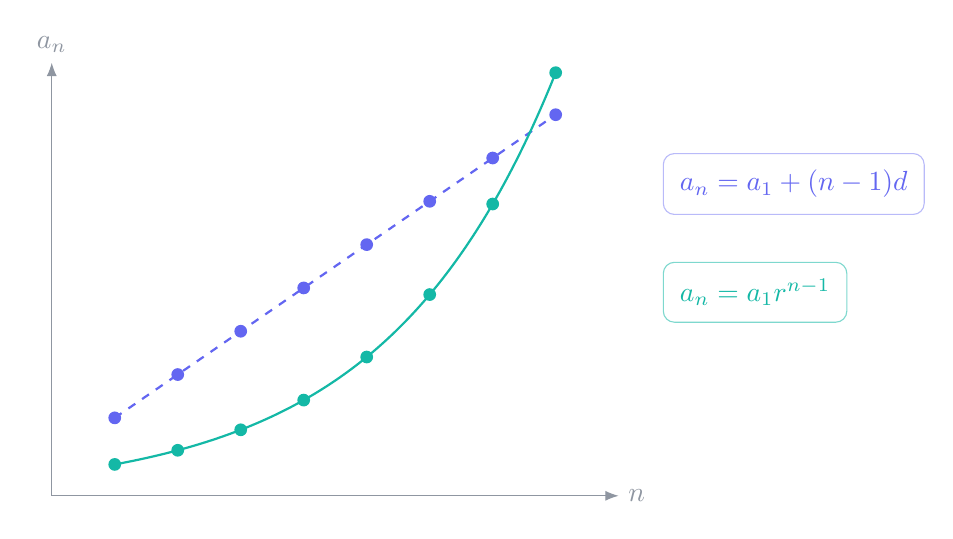
\begin{tikzpicture}[font=\sffamily,>=Latex,x=.8cm,y=.55cm]
  \draw[->,ink!55] (0,0)--(9,0) node[right] {$n$};
  \draw[->,ink!55] (0,0)--(0,10) node[above] {$a_n$};
  \foreach \n in {1,...,8} {
    \fill[nebula] (\n,{.8+\n}) circle (2.3pt);
    \fill[spark] (\n,{.5*1.45^\n}) circle (2.3pt);
  }
  \draw[nebula,thick,dashed] (1,1.8)--(8,8.8);
  \draw[spark,thick,smooth,domain=1:8,samples=80] plot(\x,{.5*1.45^\x});
  \node[nebula,draw=nebula!45,rounded corners=4pt,fill=white,inner sep=6pt,anchor=west]
    at (9.7,7.2) {$a_n=a_1+(n-1)d$};
  \node[spark,draw=spark!55,rounded corners=4pt,fill=white,inner sep=6pt,anchor=west]
    at (9.7,4.7) {$a_n=a_1r^{n-1}$};
\end{tikzpicture}
\end{document}
